%% Submissions for peer-review must enable line-numbering 
%DIF LATEXDIFF DIFFERENCE FILE


%% using the lineno option in the \documentclass command.
%%
%% Preprints and camera-ready submissions do not need 
%% line numbers, and should have this option removed.
%%
%% Please note that the line numbering option requires
%% version 1.1 or newer of the wlpeerj.cls file, and
%% the corresponding author info requires v1.2

\documentclass[fleqn,10pt,lineno]{wlpeerj} % for journal submissions
% \documentclass[fleqn,10pt]{wlpeerj} % for preprint submissions

\title{Spatial variation in allometric growth of invasive lionfish has
management implications}

\author[1]{Juan Carlos Villaseñor-Derbez}
\author[1]{Sean Fitzgerald}
\affil[1]{Bren School of Environmental Sciences and Management, University of California
  Santa Barbara, Santa Barbara, California, USA}
%DIF 21c21
%DIF < \corrauthor[1]{Juan Carlos Villaseñor-Derbez}{jvillasenor@ucsb.edu}
%DIF -------
\corrauthor[1]{Juan Carlos Villaseñor-Derbez}{juancarlos@ucsb.edu} %DIF > 
%DIF -------

\keywords{Lionfish, invasive species, length-weight, allometric, regional variations}

\begin{abstract}
Lionfish (\textit{Pterois volitans / miles}) are an invasive species in
the Western Atlantic and the Caribbean. Improving management of invasive
lionfish populations requires accurate total biomass estimates, which
depend on accurate estimates of allometric growth. Sedentary species
like lionfish often exhibit high levels of spatial variation in life
history characteristics. We review 17 published length-weight
relationships for lionfish taken throughout their invasive range and
%DIF 33-41c33-41
%DIF < found substantial regional differences in allometric growth parameters.
%DIF < The spatial pattern we observed is consistent with findings from other
%DIF < studies focusing on genetics or age-at-length. We show that the use of
%DIF < \textit{ex situ} parameters can result in up to a threefold under- or
%DIF < overestimation of total weight, but using parameters from nearby regions
%DIF < reduces this error. These findings can have major implications for
%DIF < management in terms of predicting effects on local ecosystems,
%DIF < evaluating the effectiveness of removal programs, or estimating biomass
%DIF < available for harvest.
%DIF -------
found regional differences that led to significant under- and %DIF > 
overestimation of weight estimates. The spatial pattern we observed is %DIF > 
consistent with findings from other studies focusing on genetics or %DIF > 
length-at-age. We show that the use of \textit{ex situ} parameters can %DIF > 
result in up to a threefold under- or overestimation of total weight, %DIF > 
but using parameters from nearby regions reduces this error. These %DIF > 
findings can have substantial implications for management in terms of %DIF > 
predicting effects on local ecosystems, evaluating the effectiveness of %DIF > 
removal programs, or estimating biomass available for harvest. %DIF > 
%DIF -------
\end{abstract}
%DIF PREAMBLE EXTENSION ADDED BY LATEXDIFF
%DIF UNDERLINE PREAMBLE %DIF PREAMBLE
\RequirePackage[normalem]{ulem} %DIF PREAMBLE
\RequirePackage{color}\definecolor{RED}{rgb}{1,0,0}\definecolor{BLUE}{rgb}{0,0,1} %DIF PREAMBLE
\providecommand{\DIFadd}[1]{{\protect\color{blue}\uwave{#1}}} %DIF PREAMBLE
\providecommand{\DIFdel}[1]{{\protect\color{red}\sout{#1}}}                      %DIF PREAMBLE
%DIF SAFE PREAMBLE %DIF PREAMBLE
\providecommand{\DIFaddbegin}{} %DIF PREAMBLE
\providecommand{\DIFaddend}{} %DIF PREAMBLE
\providecommand{\DIFdelbegin}{} %DIF PREAMBLE
\providecommand{\DIFdelend}{} %DIF PREAMBLE
%DIF FLOATSAFE PREAMBLE %DIF PREAMBLE
\providecommand{\DIFaddFL}[1]{\DIFadd{#1}} %DIF PREAMBLE
\providecommand{\DIFdelFL}[1]{\DIFdel{#1}} %DIF PREAMBLE
\providecommand{\DIFaddbeginFL}{} %DIF PREAMBLE
\providecommand{\DIFaddendFL}{} %DIF PREAMBLE
\providecommand{\DIFdelbeginFL}{} %DIF PREAMBLE
\providecommand{\DIFdelendFL}{} %DIF PREAMBLE
%DIF END PREAMBLE EXTENSION ADDED BY LATEXDIFF

\begin{document}

\flushbottom
\maketitle
\thispagestyle{empty}

\section*{Introduction}

Lionfish (\emph{Pterois volitans/miles} complex) are an invasive species
in the \DIFdelbegin \DIFdel{western Atlantic }\DIFdelend \DIFaddbegin \DIFadd{Western Atlantic Ocean }\DIFaddend and Caribbean Sea, likely introduced
through \DIFdelbegin \DIFdel{liberation }\DIFdelend \DIFaddbegin \DIFadd{release }\DIFaddend of aquarium-kept organisms \citep{betancurr_2011}. They
are the first invasive marine vertebrates established along \DIFdelbegin \DIFdel{the North
Atlantic Caribbean }\DIFdelend \DIFaddbegin \DIFadd{these }\DIFaddend coasts
\citep{schofield_2009,schofield_2010,sabidoitza_2016} and their presence
has been labeled as a major marine invasion because they threaten local
biodiversity, spread rapidly, and are difficult to manage
\citep{hixon_2016}. Lionfish have established invasive populations in
coral reefs, estuaries, mangroves, hard-bottomed areas, and mesophotic
reefs
\citep{barbour_2010,jud_2011,muoz_2011,claydon_2012,andradibrown_2017,gress_2017}.

A substantial amount of research describes lionfish impacts throughout
its invaded range. A meta-analysis by \citet{peake_2018} showed that
invasive lionfish prey on at least 167 different species across the
tropical and temperate \DIFdelbegin \DIFdel{North }\DIFdelend \DIFaddbegin \DIFadd{Western }\DIFaddend Atlantic. Their feeding behavior and high
consumption rates can reduce recruitment and population sizes of native
reef-fish species, and can further endanger reef fish
\DIFdelbegin \DIFdel{(\mbox{%DIFAUXCMD
\citet{green_2012,rocha_2015}}\hspace{0pt}%DIFAUXCMD
}\DIFdelend \DIFaddbegin \DIFadd{\mbox{%DIFAUXCMD
\citep{green_2012,rocha_2015}}\hspace{0pt}%DIFAUXCMD
}\DIFaddend ; but see \citet{hackerott_2017}\DIFdelbegin \DIFdel{)}\DIFdelend . For
example, field experiments by \citet{albins_2008} showed that lionfish
establishment led to reduced recruitment of native fishes by nearly 80\%
over a five-week period in \DIFdelbegin \DIFdel{Florida}\DIFdelend \DIFaddbegin \DIFadd{the Bahamas}\DIFaddend . \citet{green_2012} reported that
prey fish biomass declined by 65\% over two years as lionfish biomass
increased along Bahamian coral reefs. \DIFdelbegin \DIFdel{Their }\DIFdelend \DIFaddbegin \DIFadd{However, their }\DIFaddend trophic impacts can
be minimized if local lionfish biomass is controlled by culling
\citep{ariasgonzalez_2011}.

Governments and non-profit organizations have sought to reduce lionfish
densities through removal programs and incentivizing its consumption
\citep{chin_2016}. In some cases, these have shown to significantly
reduce --but not quite eliminate-- lionfish abundances at local scales
\citep{deleon_2013,sandel_2015}. Complete eradication of lionfish
through fishing is unlikely because of their rapid recovery rates and
ongoing recruitment to shallow-water areas from persistent populations
in mesophotic ecosystems \citep{barbour_2011,andradibrown_2017}.
However, promoting lionfish consumption might create a level of demand
capable of incentivizing a stable fishery while controlling
shallow-water populations, thus creating alternative livelihoods and
avoiding further \DIFdelbegin \DIFdel{impacts }\DIFdelend \DIFaddbegin \DIFadd{negative effects }\DIFaddend to local biota.

The feasibility of establishing fisheries through lionfish removal
programs has been extensively evaluated through field observations and
empirical modeling
\citep{barbour_2011,morris_2011,deleon_2013,johnston_2015,sandel_2015,usseglio_2017}.
Determining the feasibility of such initiatives requires modeling the
change in biomass in response to changes in fishing mortality
(\emph{i.e.} culling). A common way to model this is via
length-structured population models, where fish lengths are converted to
weight to calculate total biomass
\citep{barbour_2011,cote_2014,andradibrown_2017}. The allometric
length-weight relationship is thus an essential component of these
models, but this relationship can vary across regions as a response to
biotic and abiotic conditions \citep{johnson_2016}.

Outcomes of previous studies suggest lionfish are likely to exhibit
spatial heterogeneity in the length-weight relationship, which we
summarize in two main causes. First, culling programs are effective in
reducing local adult populations largely because lionfish exhibit high
levels of site fidelity and small home ranges
\citep{Fishelson_1997,kochzius_2005,jud_2012,cote_2014}. It is \DIFdelbegin \DIFdel{know }\DIFdelend \DIFaddbegin \DIFadd{known
}\DIFaddend that fish with sedentary behavior are likely to exhibit high levels of
spatial variation in important life history \DIFdelbegin \DIFdel{characterstics }\DIFdelend \DIFaddbegin \DIFadd{characteristics }\DIFaddend such as
growth or natural mortality rates
\citep{gunderson_2008,hutchinson_2008,wilson_2012,guan_2013}. Second,
genetic analysis of lionfish suggests biological differences due to the
existence of two genetically distinct invasive subpopulations between
the \DIFdelbegin \DIFdel{northwest }\DIFdelend \DIFaddbegin \DIFadd{Western }\DIFaddend Atlantic and the Caribbean \citep{betancurr_2011}. \DIFdelbegin \DIFdel{Site-specific parameters are necessary to accurately estimate biomass
when allometric relationships are spatially variable , and this
variability is }\DIFdelend \DIFaddbegin \DIFadd{The large
number of site-specific studies reporting the length-weight relationship
of lionfish provide variable estimates. These differences may be
}\DIFaddend increasingly important when estimating the potential effectiveness of
lionfish culling programs
\citep{barbour_2011,morris_2011,cote_2014,johnston_2015}. However, the
\DIFdelbegin \DIFdel{region-wide differences in allometric growth parameters has remained
unexplored for lionfish, despite the large number of site-specific
studies reporting the length-weight relationship}\DIFdelend \DIFaddbegin \DIFadd{magnitude of the error caused by using }\emph{\DIFadd{ex situ}} \DIFadd{parameters to
estimate total weight from length observations remains unexplored}\DIFaddend .

Here, we \DIFdelbegin \DIFdel{compare }\DIFdelend \DIFaddbegin \DIFadd{use }\DIFaddend previously published length-weight relationships for
lionfish populations in North Carolina, Northern and Southern Gulf of
Mexico, the Southern Mexican Caribbean, Bahamas, Little Cayman, Jamaica,
Bonaire, Puerto Rico, and Costa Rica \DIFdelbegin \DIFdel{\mbox{%DIFAUXCMD
\citep{barbour_2011,darling_2011,deleon_2013,fogg_2013,dahl_2014,edwards_2014,toledohernndez_2014,sandel_2015,aguilarperera_2016,sabidoitza_2016,sabidoitz_2016,chin_2016}}\hspace{0pt}%DIFAUXCMD
}\DIFdelend \DIFaddbegin \DIFadd{to quantify the magnitude of the
error caused by using }\emph{\DIFadd{ex situ}} \DIFadd{parameters to estimate lionfish
weight from length observations}\DIFaddend . We also collected lionfish length and
weight data in the central Mexican Caribbean and report the first
\DIFdelbegin \DIFdel{allometric growth equation }\DIFdelend \DIFaddbegin \DIFadd{length-weight relationship }\DIFaddend for this region.
\DIFdelbegin \DIFdel{The objective of this paper is to describe the spatial pattern
of length-weight relationships of lionfish across the Caribbean and
Western Atlantic and to discuss implications of these spatial
differences.
}\DIFdelend 

\clearpage

\section*{Methods}

We reviewed 12 published studies and obtained 17 length-weight
relationships for the \DIFdelbegin \DIFdel{North }\DIFdelend \DIFaddbegin \DIFadd{Western }\DIFaddend Atlantic (n = \DIFdelbegin \DIFdel{1}\DIFdelend \DIFaddbegin \DIFadd{2}\DIFaddend ), Gulf of Mexico (n = 7),
and Caribbean (n = \DIFdelbegin \DIFdel{9}\DIFdelend \DIFaddbegin \DIFadd{8}\DIFaddend , Table \ref{tab:all_params}, Fig \DIFdelbegin \DIFdel{\ref{fig:all_allo}}\DIFdelend \DIFaddbegin \DIFadd{\ref{fig:map}}\DIFaddend ). We
collected information on \DIFdelbegin \DIFdel{sampling methods, }\DIFdelend sex differentiation, location, \DIFaddbegin \DIFadd{length }\DIFaddend and depth
ranges \DIFaddbegin \DIFadd{and sampling methods }\DIFaddend from each study when available. Only two
studies reported parameters for each gender
\citep{aguilarperera_2016,fogg_2013}, so we assumed both genders were
included in a study if gender was unspecified. Reviewed studies
presented information for organisms \DIFaddbegin \DIFadd{ranging between 25 mm and 475 mm in
Total Length (\(TL\)), and that were }\DIFaddend obtained at depths between 0.5 m
and 57 m. \DIFdelbegin \DIFdel{Three }\DIFdelend \DIFaddbegin \DIFadd{Four }\DIFaddend studies explicitly stated that their organisms were
sampled with pole spears
\citep{dahl_2014,aguilarperera_2016,chin_2016,sabidoitz_2016}, and \DIFdelbegin \DIFdel{five
}\DIFdelend \DIFaddbegin \DIFadd{six
}\DIFaddend studies mentioned that some of their organisms were obtained with pole
spears (or other type of harpoon) but also hand-held nets or fish traps
\DIFdelbegin \DIFdel{\mbox{%DIFAUXCMD
\citep{barbour_2011,fogg_2013,edwards_2014,toledohernndez_2014,sandel_2015,sabidoitza_2016,sabidoitz_2016}}\hspace{0pt}%DIFAUXCMD
}\DIFdelend \DIFaddbegin \DIFadd{\mbox{%DIFAUXCMD
\citep{barbour_2011,fogg_2013,edwards_2014,toledohernndez_2014,sandel_2015,sabidoitza_2016}}\hspace{0pt}%DIFAUXCMD
}\DIFaddend ,
and two studies did not specify how organisms were sampled
\citep{darling_2011,deleon_2013}.
\DIFdelbegin \DIFdel{\mbox{%DIFAUXCMD
\citet{fogg_2013} }\hspace{0pt}%DIFAUXCMD
use spineless weight
in their calculations, so their parameters likely underestimated total
wieght. Since no spineless to total weight conversions were available,
these parameters were taken as reported.
}\DIFdelend 

\begin{figure}
\centering
\DIFdelbeginFL %DIFDELCMD < 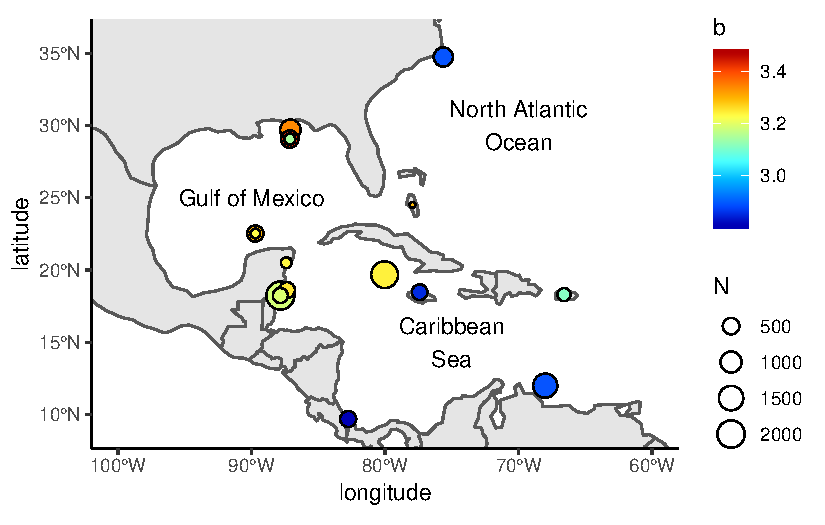
\includegraphics{Manuscript_files/figure-latex/unnamed-chunk-2-1.pdf}
%DIFDELCMD < %%%
\DIFdelendFL \DIFaddbeginFL 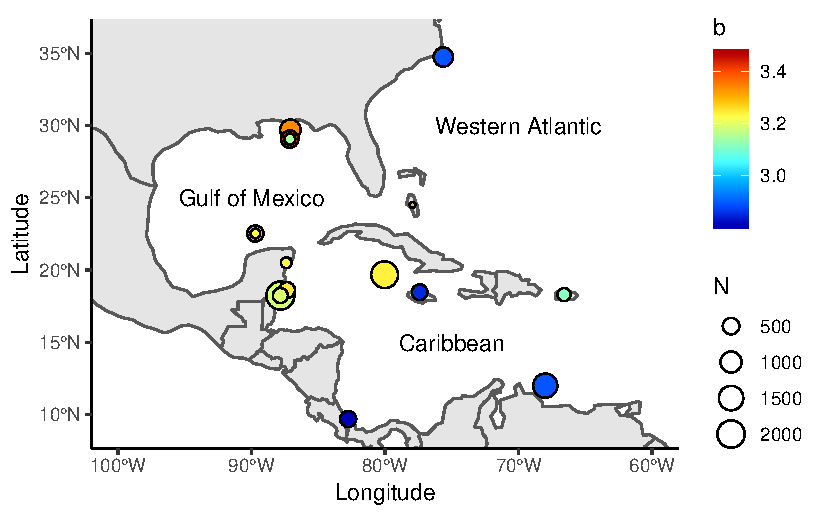
\includegraphics{Manuscript_files/figure-latex/map-1.pdf}
\DIFaddendFL \caption{\label{fig:map}Locations where allometric growth parameters of
lionfish (\emph{Pterois spp}) have been reported. Circle sizes indicate
sample size from each study, colors indicate the \(b\) coefficient from
Eq. \ref{eq:allometric}.}
\end{figure}

We also \DIFdelbegin \DIFdel{collected data from }\DIFdelend \DIFaddbegin \DIFadd{used data from \mbox{%DIFAUXCMD
\citet{villaseorderbez_2014}}\hspace{0pt}%DIFAUXCMD
, who collected
organisms from }\DIFaddend 10 sampling sites along the central Mexican Caribbean
coast in \DIFaddbegin \DIFadd{the Summer of }\DIFaddend 2010 (Supplementary Table 1). Sampling locations
included wall and carpet reefs at depths between 5.7 m and 38.1 m. All
observed lionfish (n = 109) were collected using hand nets and numbered
collection bottles. The use of hand nets prevented any weight loss due
to bleeding and allowed better representation of small sizes by \DIFdelbegin \DIFdel{eliminating }\DIFdelend \DIFaddbegin \DIFadd{avoiding
}\DIFaddend gear selectivity. Organisms were euthanized via pithing and Total Length
(TL; mm) and Total Weight (TW; g) were recorded.

\DIFaddbegin \clearpage

\DIFaddend The weight-at-length relationship for lionfish in the central Mexican
Caribbean was calculated with the allometric growth function:

\begin{equation}
\label{eq:allometric}
TW = aTL^b
\end{equation}

Where \(a\) is the ponderal index and \(b\) is the scaling exponent or
allometric parameter.

\DIFdelbegin %DIFDELCMD < \clearpage
%DIFDELCMD < 

%DIFDELCMD < %%%
\DIFdel{Transforming this equation via base-10 logarithms we obtain:
}%DIFDELCMD < 

%DIFDELCMD < %%%
\begin{displaymath}
\DIFdel{%DIFDELCMD < \label{eq:log-alo}%%%
log_{10}(TW) = b\times log_{10}(TL) + log_{10}(a)
}\end{displaymath}%DIFAUXCMD
%DIFDELCMD < 

%DIFDELCMD < %%%
\DIFdel{This can be simplified and re-written as:
}%DIFDELCMD < 

%DIFDELCMD < %%%
\begin{displaymath}
\DIFdel{%DIFDELCMD < \label{eq:log-alo-trans}%%%
Y = bX + c
}\end{displaymath}%DIFAUXCMD
%DIFDELCMD < 

%DIFDELCMD < %%%
\DIFdel{Where \(Y = log_{10}(TW)\), \(X = log_{10}(TL)\), and
\(c = log_{10}(a)\)}\DIFdelend \DIFaddbegin \DIFadd{The above equation was linearized using \(log_{10}\)-transformation}\DIFaddend . The
coefficients \DIFdelbegin \DIFdel{(\(c\) and \(b\)) }\DIFdelend were estimated with an Ordinary Least Squares Regression\DIFaddbegin \DIFadd{,
}\DIFaddend and heteroskedastic-robust standard error correction \DIFaddbegin \DIFadd{was applied
}\DIFaddend \citep{zeileis_2004}. When \DIFdelbegin \DIFdel{the }\DIFdelend \(b = 3\), it is said that the organism
exhibits a perfect isometric growth, so the \(b\) coefficient was tested
against the null hypothesis of isometric growth (\emph{i.e.}
\(H_0: b = 3\)). Coefficients were tested with a two-tailed Student's t,
and the significance of the regression was corroborated with an F-test.

Some of the reviewed studies inconsistently defined \(a\) as either the
ponderal index from Eq. \ref{eq:allometric} or the y-intercept \DIFdelbegin \DIFdel{(\(c\))
from Eq. \ref{eq:log-alo-trans}. }\DIFdelend \DIFaddbegin \DIFadd{from the
linearized log-transformed equation. }\DIFaddend Other studies incorrectly reported
parameters as mm-to-g conversions when they were in fact cm-to-g
conversions. We standardized each study by converting coefficients and
report all parameters as TL (mm) to TW (\DIFdelbegin \DIFdel{gr}\DIFdelend \DIFaddbegin \DIFadd{g}\DIFaddend ) conversions. Locations where
allometric studies have been performed are shown in Figure \ref{fig:map}
and summarized in Table \ref{tab:all_params}.

We obtained a total of 18 parameter pairs by combining length-weight
parameters extracted from the literature and the additional pair
calculated here. \DIFaddbegin \DIFadd{Recall that the objective of this study is not to
describe variations between populations, but rather to estimate how the
use of }\emph{\DIFadd{ex situ}} \DIFadd{parameters influences weight estimates. }\DIFaddend We used
the central Mexican Caribbean as a case study of how the use of \emph{ex
situ} parameters influences the accuracy of weight estimates for
lionfish. We estimated \DIFdelbegin \DIFdel{TW from the TL }\DIFdelend \DIFaddbegin \DIFadd{\(TW\) from the \(TL\) }\DIFaddend observations we collected
in the central Mexican Caribbean (n = 109, with \DIFdelbegin \DIFdel{\(TL \in (34, 310)\)}\DIFdelend \DIFaddbegin \DIFadd{\(TL\) ranging from 34
mm to 310 mm}\DIFaddend ) using each of the 18 parameter pairs and divided predicted
weights by known observed weights to obtain a simple measure of over- or
underestimation. Difference in mean weight ratios \DIFdelbegin \DIFdel{across the
different parameter pairs }\DIFdelend were tested with \DIFdelbegin \DIFdel{a one-way analysis of variance (ANOVA)and }\DIFdelend \DIFaddbegin \DIFadd{an
analysis of covariance (ANCOVA), where the sources of variation were the
study and \(TL\). Ratios were logit-transformed prior to analysis, and a
}\emph{\DIFadd{post-hoc}} \DIFaddend Tukey's test was used \DIFdelbegin \DIFdel{for }\emph{\DIFdel{post-hoc}} %DIFAUXCMD
\DIFdel{tests}\DIFdelend \DIFaddbegin \DIFadd{to identify groups where mean
ratios did not differ}\DIFaddend . All analyses were performed in R version 3.5\DIFdelbegin \DIFdel{.1 }\DIFdelend \DIFaddbegin \DIFadd{.2
}\DIFaddend \citep{rcore_2018}. Raw data and code used in this work are available on
github \DIFdelbegin \DIFdel{.
}\DIFdelend \DIFaddbegin \DIFadd{at github.com/jcvdav/lionfish\_biometry.
}\DIFaddend 

\section*{Results}

The length-weight relationship for organisms from the central Mexican
Caribbean resulted in \DIFdelbegin \DIFdel{the coefficient values }\DIFdelend \DIFaddbegin \DIFadd{coefficient values of
}\DIFaddend \(a = 3.2056297\times 10^{-6}\) \DIFdelbegin \DIFdel{, \(b = 3.2347391\) and \(c = -5.4940866\) }\DIFdelend \DIFaddbegin \DIFadd{and \(b = 3.2347391\) }\DIFaddend (\(R^2 = 0.977\),
F(df = 1; 107) = 6928.67, \(p < 0.001\)). The allometric factor (\(b\))
was significantly different from \(b = 3\) (\(t(107) = 6.04; p<0.001\))
\DIFdelbegin \DIFdel{indicating }\DIFdelend \DIFaddbegin \DIFadd{corroborating }\DIFaddend that lionfish present allometric growth. The length-weight
coefficients estimated in this study were within the range identified by
studies in other regions (Table \ref{tab:all_params}). Figure
\ref{fig:l-w-carib} shows the relationship between TL and TW for this
region\DIFdelbegin \DIFdel{, and model fit
statistics are presented in Table \ref{tab:reg_table}}\DIFdelend .

\begin{figure}
\centering
\DIFdelbeginFL %DIFDELCMD < 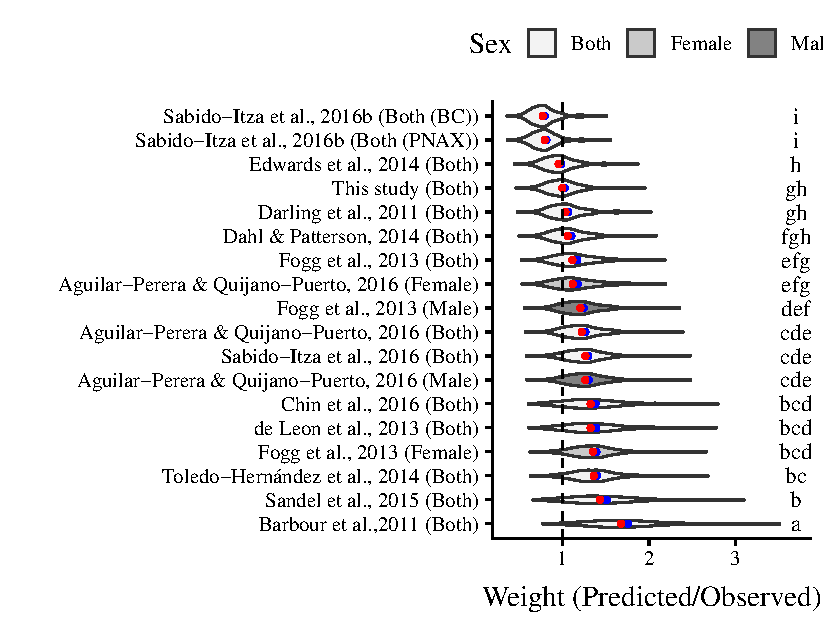
\includegraphics{Manuscript_files/figure-latex/unnamed-chunk-7-1.pdf}
%DIFDELCMD < %%%
\DIFdelendFL \DIFaddbeginFL 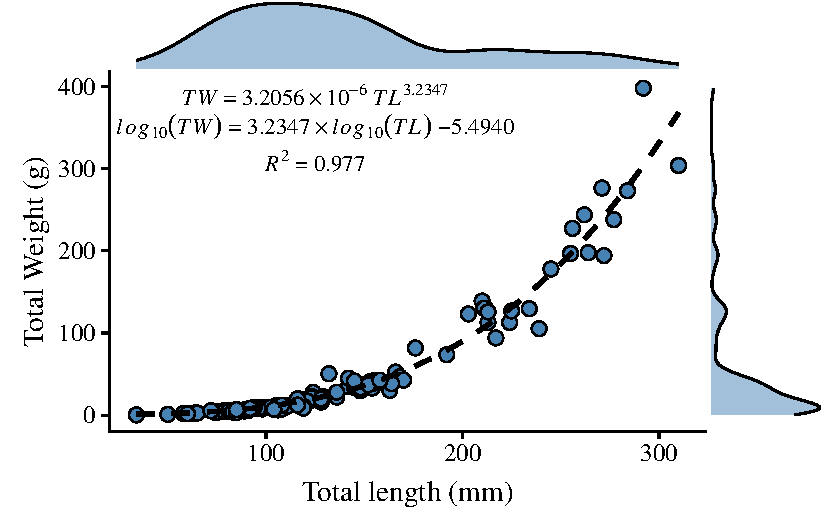
\includegraphics{Manuscript_files/figure-latex/fit1-1.pdf}
\DIFaddendFL \caption{\label{fig:l-w-carib}Length-weight relationship for 109
lionfish sampled in the central Mexican Caribbean. Points indicate
samples, dashed black line indicates curve of best fit, marginal plots
represent the density distribution of each variable.}
\end{figure}

\DIFdelbegin %DIFDELCMD < \begin{table}[!htbp] \centering 
%DIFDELCMD <   %%%
%DIFDELCMD < \caption{%
{%DIFAUXCMD
%DIFDELCMD < \label{tab:reg_table}%%%
\DIFdelFL{Coefficients of the linear model fit to Eq \ref{eq:log-alo-trans}. Numbers in parenthesees represent heteroskedastic-robust standard errors.}} 
  %DIFAUXCMD
%DIFDELCMD < \label{} 
%DIFDELCMD < \begin{tabular}{@{\extracolsep{5pt}}lc} 
%DIFDELCMD < \\[-1.8ex]\hline 
%DIFDELCMD < \hline \\[-1.8ex] 
%DIFDELCMD <  & \multicolumn{1}{c}{$log_{10}(TW)$} \\ 
%DIFDELCMD < \cline{2-2} 
%DIFDELCMD < \hline \\[-1.8ex] 
%DIFDELCMD <  %%%
\DIFdelFL{c }%DIFDELCMD < & %%%
\DIFdelFL{$-$5.494 (0.083)$^{***}$ }%DIFDELCMD < \\ 
%DIFDELCMD <   %%%
\DIFdelFL{b }%DIFDELCMD < & %%%
\DIFdelFL{3.235 (0.039)$^{***}$ }%DIFDELCMD < \\ 
%DIFDELCMD <  \hline \\[-1.8ex] 
%DIFDELCMD < %%%
\DIFdelFL{F Statistic }%DIFDELCMD < & %%%
\DIFdelFL{6928.67*** (df = 1; 107) }%DIFDELCMD < \\ 
%DIFDELCMD < %%%
\DIFdelFL{Observations }%DIFDELCMD < & %%%
\DIFdelFL{109 }%DIFDELCMD < \\ 
%DIFDELCMD < %%%
\DIFdelFL{Adjusted R$^{2}$ }%DIFDELCMD < & %%%
\DIFdelFL{0.976 }%DIFDELCMD < \\ 
%DIFDELCMD < %%%
\DIFdelFL{Residual Std. Error }%DIFDELCMD < & %%%
\DIFdelFL{0.096 (df = 107) }%DIFDELCMD < \\ 
%DIFDELCMD < \hline 
%DIFDELCMD < \hline \\[-1.8ex] 
%DIFDELCMD < %%%
\textit{\DIFdelFL{Note:}}  %DIFAUXCMD
%DIFDELCMD < & \multicolumn{1}{r}{$^{*}$p$<$0.1; $^{**}$p$<$0.05; $^{***}$p$<$0.01} \\ 
%DIFDELCMD < \end{tabular} 
%DIFDELCMD < \end{table}
%DIFDELCMD < 

%DIFDELCMD < %%%
\DIFdelend There were significant differences in our predicted weights for the
central Mexican Caribbean when using \DIFaddbegin \DIFadd{each of }\DIFaddend the different pairs of
parameters (\DIFdelbegin \DIFdel{\(F(df = 17; 1944) = 61.55; p < 0.001\)}\DIFdelend \DIFaddbegin \DIFadd{\(F(df = 17; 1943) = 24.96; p < 0.001\)}\DIFaddend ). The lowest weight
estimates \DIFaddbegin \DIFadd{for the observed lengths }\DIFaddend resulted from using the allometric
parameters from Banco Chinchorro in the Caribbean, with mean \(\pm\) SD
of 40.37 \(\pm\) 58.74 \DIFdelbegin \DIFdel{gr
\mbox{%DIFAUXCMD
\citep{sabidoitz_2016}}\hspace{0pt}%DIFAUXCMD
, and }\DIFdelend \DIFaddbegin \DIFadd{g \mbox{%DIFAUXCMD
\citep{sabidoitz_2016}}\hspace{0pt}%DIFAUXCMD
. In contrast, }\DIFaddend the
highest weight estimates came from the \DIFdelbegin \DIFdel{Northern }\DIFdelend \DIFaddbegin \DIFadd{Western }\DIFaddend Atlantic with 73.76
\(\pm\) 96.11 \DIFdelbegin \DIFdel{gr }\DIFdelend \DIFaddbegin \DIFadd{g }\DIFaddend \citep{barbour_2011}. To put this in context, true
observed weights \DIFdelbegin \DIFdel{were }\DIFdelend \DIFaddbegin \DIFadd{have a mean of }\DIFaddend 52.56 \(\pm\) 76.58 \DIFdelbegin \DIFdel{gr. These correspond to }\DIFdelend \DIFaddbegin \DIFadd{g. Weights predicted
from these extreme parameters correspond to mean \(\pm\) SD
}\DIFaddend predicted-to-observed weights ratios of 0.80 \(\pm\) 0.19 and 1.76
\(\pm\) 0.50 (mean \(\pm\) SD), respectively. \DIFdelbegin %DIFDELCMD < 

%DIFDELCMD < %%%
\DIFdel{The calculated ratio of predicted-to-observed weight ranged from }\DIFdelend \DIFaddbegin \DIFadd{The largest under- and
overestimations resulted in ratios of }\DIFaddend 0.36 \DIFdelbegin \DIFdel{to
}\DIFdelend \DIFaddbegin \DIFadd{and }\DIFaddend 3.51 \DIFaddbegin \DIFadd{of the actual
observed weight}\DIFaddend , indicating that \emph{ex situ} parameters can result in
\DIFdelbegin \DIFdel{major
}\DIFdelend \DIFaddbegin \DIFadd{substantial weight }\DIFaddend under- and \DIFdelbegin \DIFdel{overestimations.
}\DIFdelend \DIFaddbegin \DIFadd{overestimation.
}

\DIFaddend Tukey's \emph{post-hoc} test suggests that weight ratios for the central
Mexican Caribbean were not different from those obtained with parameters
from Little Cayman, the Bahamas, and some sites in the Gulf of Mexico
(\DIFdelbegin \DIFdel{Tukeys }\DIFdelend \DIFaddbegin \DIFadd{Tukey's }\DIFaddend HSD \(p > 0.05\)). Weight estimates using parameters from the
Gulf of Mexico and \DIFdelbegin \DIFdel{North-Western }\DIFdelend \DIFaddbegin \DIFadd{Western }\DIFaddend Atlantic were higher on average than those
from the Caribbean (Fig \ref{fig:all_allo}). The average (\(\pm\) SD)
predicted-to-observed weight ratios from these three regions were 1.24
\(\pm\) 0.309, 1.76 \(\pm\) 0.496, and 1.17 \(\pm\) 0.398, respectively.
\DIFaddbegin \DIFadd{This suggest that the smallest errors are observed when using parameters
other locations in the Caribbean. }\DIFaddend Predicted-to-observed weight ratios
are presented in Figure \ref{fig:bio_ratio}.
\DIFdelbegin \DIFdel{Spineless weight parameters from \mbox{%DIFAUXCMD
\citet{fogg_2013}
}\hspace{0pt}%DIFAUXCMD
still produced predicted-to-observed weight ratios \textgreater{} 1.
}\DIFdelend 

\DIFdelbegin %DIFDELCMD < \begin{table}
%DIFDELCMD < %%%
\DIFdelendFL \DIFaddbeginFL \begin{table}[t]
\DIFaddendFL 

\caption{\DIFdelbeginFL %DIFDELCMD < \label{tab:unnamed-chunk-9}%%%
\DIFdelendFL \DIFaddbeginFL \label{tab:unnamed-chunk-7}\DIFaddendFL \label{tab:all_params}Summary of 18 allometric growth parameters available for lionfish in the invaded range from peer-reviewed literature and this study. All parameters have been adjusted to convert from millimeters to grams. n = Sample size, Sex specifies whether data was presented for Females (F), Males (M), or both genders combined (B), a = scaling parameter \DIFdelbeginFL \DIFdelFL{for Eq. 1 }\DIFdelendFL (presented in $\times 10^{-5}$), \DIFdelbeginFL \DIFdelFL{c = y-intercept for Eq. 3, }\DIFdelendFL b = exponent\DIFdelbeginFL \DIFdelFL{or slope for Eq}\DIFdelendFL .\DIFdelbeginFL \DIFdelFL{1 or Eq. 3, respectively. The Fit column contains the reported $R^2$ of the model fit.}\DIFdelendFL }
\centering
\DIFdelbeginFL %DIFDELCMD < \begin{tabular}[t]{llllrrll}
%DIFDELCMD < %%%
\DIFdelendFL \DIFaddbeginFL \begin{tabular}{llllrll}
\DIFaddendFL \toprule
Region & Sex & n & a & b & \DIFdelbeginFL \DIFdelFL{c }\DIFdelendFL \DIFaddbeginFL \DIFaddFL{$R^2$ }\DIFaddendFL & \DIFdelbeginFL \DIFdelFL{Fit }%DIFDELCMD < & %%%
\DIFdelendFL Reference\\
\midrule
\DIFdelbeginFL \DIFdelFL{Caribbean }\DIFdelendFL \DIFaddbeginFL \DIFaddFL{Western Atlantic }\DIFaddendFL & B & \DIFdelbeginFL \DIFdelFL{458 }\DIFdelendFL \DIFaddbeginFL \DIFaddFL{774 }\DIFaddendFL & \DIFdelbeginFL \DIFdelFL{3.6 }\DIFdelendFL \DIFaddbeginFL \DIFaddFL{2.9 }\DIFaddendFL & \DIFdelbeginFL \DIFdelFL{2.81 }\DIFdelendFL \DIFaddbeginFL \DIFaddFL{2.89 }\DIFaddendFL & \DIFdelbeginFL \DIFdelFL{-4.44 }%DIFDELCMD < & %%%
\DIFdelendFL - & \DIFdelbeginFL \DIFdelFL{Sandel }\DIFdelendFL \DIFaddbeginFL \DIFaddFL{Barbour }\DIFaddendFL et al., \DIFdelbeginFL \DIFdelFL{2015}\DIFdelendFL \DIFaddbeginFL \DIFaddFL{2011}\DIFaddendFL \\
\DIFdelbeginFL \DIFdelFL{Caribbean }\DIFdelendFL \DIFaddbeginFL \DIFaddFL{Western Atlantic }\DIFaddendFL & B & \DIFdelbeginFL \DIFdelFL{419 }\DIFdelendFL \DIFaddbeginFL \DIFaddFL{- }\DIFaddendFL & \DIFdelbeginFL \DIFdelFL{2.8 }\DIFdelendFL \DIFaddbeginFL \DIFaddFL{0.25 }\DIFaddendFL & \DIFdelbeginFL \DIFdelFL{2.85 }\DIFdelendFL \DIFaddbeginFL \DIFaddFL{3.29 }\DIFaddendFL & \DIFdelbeginFL \DIFdelFL{-4.56 }\DIFdelendFL \DIFaddbeginFL \DIFaddFL{- }\DIFaddendFL & \DIFdelbeginFL \DIFdelFL{0.8715 }%DIFDELCMD < & %%%
\DIFdelFL{Chin }\DIFdelendFL \DIFaddbeginFL \DIFaddFL{Darling }\DIFaddendFL et al., \DIFdelbeginFL \DIFdelFL{2016}\DIFdelendFL \DIFaddbeginFL \DIFaddFL{2011}\DIFaddendFL \\
\DIFdelbeginFL \DIFdelFL{Caribbean }\DIFdelendFL \DIFaddbeginFL \DIFaddFL{GoM }\DIFaddendFL & B & \DIFdelbeginFL \DIFdelFL{1450 }\DIFdelendFL \DIFaddbeginFL \DIFaddFL{934 }\DIFaddendFL & \DIFdelbeginFL \DIFdelFL{2.3 }\DIFdelendFL \DIFaddbeginFL \DIFaddFL{0.21 }\DIFaddendFL & \DIFdelbeginFL \DIFdelFL{2.89 }\DIFdelendFL \DIFaddbeginFL \DIFaddFL{3.34 }\DIFaddendFL & \DIFdelbeginFL \DIFdelFL{-4.64 }\DIFdelendFL \DIFaddbeginFL \DIFaddFL{0.98 }\DIFaddendFL & \DIFdelbeginFL \DIFdelFL{0.96 }%DIFDELCMD < & %%%
\DIFdelFL{de Leon et al., 2013}\DIFdelendFL \DIFaddbeginFL \DIFaddFL{Dahl \& Patterson, 2014}\DIFaddendFL \\
\DIFdelbeginFL \DIFdelFL{Caribbean }\DIFdelendFL \DIFaddbeginFL \DIFaddFL{GoM }\DIFaddendFL & B & \DIFdelbeginFL \DIFdelFL{1887 }\DIFdelendFL \DIFaddbeginFL \DIFaddFL{472 }\DIFaddendFL & \DIFdelbeginFL \DIFdelFL{0.3 }\DIFdelendFL \DIFaddbeginFL \DIFaddFL{0.29 }\DIFaddendFL & \DIFdelbeginFL \DIFdelFL{3.24 }\DIFdelendFL \DIFaddbeginFL \DIFaddFL{3.30 }\DIFaddendFL & \DIFdelbeginFL \DIFdelFL{-5.52 }\DIFdelendFL \DIFaddbeginFL \DIFaddFL{0.95 }\DIFaddendFL & \DIFdelbeginFL \DIFdelFL{0.97 }%DIFDELCMD < & %%%
\DIFdelFL{Edwards et al., 2014}\DIFdelendFL \DIFaddbeginFL \DIFaddFL{Aguilar-Perera \& Quijano-Puerto, 2016}\DIFaddendFL \\
\DIFdelbeginFL \DIFdelFL{Caribbean }\DIFdelendFL \DIFaddbeginFL \DIFaddFL{GoM }\DIFaddendFL & \DIFdelbeginFL \DIFdelFL{B }\DIFdelendFL \DIFaddbeginFL \DIFaddFL{F }\DIFaddendFL & \DIFdelbeginFL \DIFdelFL{- }\DIFdelendFL \DIFaddbeginFL \DIFaddFL{67 }\DIFaddendFL & \DIFdelbeginFL \DIFdelFL{0.25 }\DIFdelendFL \DIFaddbeginFL \DIFaddFL{0.12 }\DIFaddendFL & \DIFdelbeginFL \DIFdelFL{3.29 }\DIFdelendFL \DIFaddbeginFL \DIFaddFL{3.47 }\DIFaddendFL & \DIFdelbeginFL \DIFdelFL{-5.60 }\DIFdelendFL \DIFaddbeginFL \DIFaddFL{0.95 }\DIFaddendFL & \DIFdelbeginFL \DIFdelFL{- }%DIFDELCMD < & %%%
\DIFdelFL{Darling et al., 2011}\DIFdelendFL \DIFaddbeginFL \DIFaddFL{Aguilar-Perera \& Quijano-Puerto, 2016}\DIFaddendFL \\
\addlinespace
\DIFdelbeginFL \DIFdelFL{Caribbean }\DIFdelendFL \DIFaddbeginFL \DIFaddFL{GoM }\DIFaddendFL & \DIFdelbeginFL \DIFdelFL{B }\DIFdelendFL \DIFaddbeginFL \DIFaddFL{M }\DIFaddendFL & \DIFdelbeginFL \DIFdelFL{2143 }\DIFdelendFL \DIFaddbeginFL \DIFaddFL{59 }\DIFaddendFL & \DIFdelbeginFL \DIFdelFL{0.52 }\DIFdelendFL \DIFaddbeginFL \DIFaddFL{0.42 }\DIFaddendFL & \DIFdelbeginFL \DIFdelFL{3.18 }\DIFdelendFL \DIFaddbeginFL \DIFaddFL{3.23 }\DIFaddendFL & \DIFdelbeginFL \DIFdelFL{-5.28 }\DIFdelendFL \DIFaddbeginFL \DIFaddFL{0.95 }\DIFaddendFL & \DIFdelbeginFL \DIFdelFL{0.9907 }%DIFDELCMD < & %%%
\DIFdelFL{Sabido-Itza et al.}\DIFdelendFL \DIFaddbeginFL \DIFaddFL{Aguilar-Perera \& Quijano-Puerto}\DIFaddendFL , 2016\\
\DIFdelbeginFL \DIFdelFL{Caribbean }\DIFdelendFL \DIFaddbeginFL \DIFaddFL{GoM }\DIFaddendFL & B & \DIFdelbeginFL \DIFdelFL{227 }\DIFdelendFL \DIFaddbeginFL \DIFaddFL{582 }\DIFaddendFL & \DIFdelbeginFL \DIFdelFL{0.8 }\DIFdelendFL \DIFaddbeginFL \DIFaddFL{0.14 }\DIFaddendFL & \DIFdelbeginFL \DIFdelFL{3.11 }\DIFdelendFL \DIFaddbeginFL \DIFaddFL{3.43 }\DIFaddendFL & \DIFdelbeginFL \DIFdelFL{-5.10 }\DIFdelendFL \DIFaddbeginFL \DIFaddFL{0.99 }\DIFaddendFL & \DIFdelbeginFL \DIFdelFL{0.958 }%DIFDELCMD < & %%%
\DIFdelFL{Toledo-Hernández }\DIFdelendFL \DIFaddbeginFL \DIFaddFL{Fogg }\DIFaddendFL et al., \DIFdelbeginFL \DIFdelFL{2014}\DIFdelendFL \DIFaddbeginFL \DIFaddFL{2013}\DIFaddendFL \\
\DIFdelbeginFL \DIFdelFL{Caribbean }\DIFdelendFL \DIFaddbeginFL \DIFaddFL{GoM }\DIFaddendFL & \DIFdelbeginFL \DIFdelFL{B }\DIFdelendFL \DIFaddbeginFL \DIFaddFL{M }\DIFaddendFL & \DIFdelbeginFL \DIFdelFL{449 }\DIFdelendFL \DIFaddbeginFL \DIFaddFL{119 }\DIFaddendFL & \DIFdelbeginFL \DIFdelFL{0.23 }\DIFdelendFL \DIFaddbeginFL \DIFaddFL{0.27 }\DIFaddendFL & \DIFdelbeginFL \DIFdelFL{3.25 }\DIFdelendFL \DIFaddbeginFL \DIFaddFL{3.31 }\DIFaddendFL & \DIFdelbeginFL \DIFdelFL{-5.64 }%DIFDELCMD < & %%%
\DIFdelendFL 0.97 & \DIFdelbeginFL \DIFdelFL{Sabido-Itza }\DIFdelendFL \DIFaddbeginFL \DIFaddFL{Fogg }\DIFaddendFL et al., \DIFdelbeginFL \DIFdelFL{2016b}\DIFdelendFL \DIFaddbeginFL \DIFaddFL{2013}\DIFaddendFL \\
\DIFdelbeginFL \DIFdelFL{Caribbean }\DIFdelendFL \DIFaddbeginFL \DIFaddFL{GoM }\DIFaddendFL & \DIFdelbeginFL \DIFdelFL{B }\DIFdelendFL \DIFaddbeginFL \DIFaddFL{F }\DIFaddendFL & \DIFdelbeginFL \DIFdelFL{368 }\DIFdelendFL \DIFaddbeginFL \DIFaddFL{115 }\DIFaddendFL & \DIFdelbeginFL \DIFdelFL{0.32 }\DIFdelendFL \DIFaddbeginFL \DIFaddFL{0.68 }\DIFaddendFL & \DIFdelbeginFL \DIFdelFL{3.19 }\DIFdelendFL \DIFaddbeginFL \DIFaddFL{3.14 }\DIFaddendFL & \DIFdelbeginFL \DIFdelFL{-5.50 }\DIFdelendFL \DIFaddbeginFL \DIFaddFL{0.94 }\DIFaddendFL & \DIFdelbeginFL \DIFdelFL{0.98 }%DIFDELCMD < & %%%
\DIFdelFL{Sabido-Itza }\DIFdelendFL \DIFaddbeginFL \DIFaddFL{Fogg }\DIFaddendFL et al., \DIFdelbeginFL \DIFdelFL{2016b}\DIFdelendFL \DIFaddbeginFL \DIFaddFL{2013}\DIFaddendFL \\
Caribbean & B & \DIFdelbeginFL \DIFdelFL{109 }\DIFdelendFL \DIFaddbeginFL \DIFaddFL{458 }\DIFaddendFL & \DIFdelbeginFL \DIFdelFL{0.32 }\DIFdelendFL \DIFaddbeginFL \DIFaddFL{3.6 }\DIFaddendFL & \DIFdelbeginFL \DIFdelFL{3.23 }\DIFdelendFL \DIFaddbeginFL \DIFaddFL{2.81 }\DIFaddendFL & \DIFdelbeginFL \DIFdelFL{-5.49 }\DIFdelendFL \DIFaddbeginFL \DIFaddFL{- }\DIFaddendFL & \DIFdelbeginFL \DIFdelFL{0.9766 }%DIFDELCMD < & %%%
\DIFdelFL{This study}\DIFdelendFL \DIFaddbeginFL \DIFaddFL{Sandel et al., 2015}\DIFaddendFL \\
\addlinespace
\DIFdelbeginFL \DIFdelFL{GoM }\DIFdelendFL \DIFaddbeginFL \DIFaddFL{Caribbean }\DIFaddendFL & B & \DIFdelbeginFL \DIFdelFL{934 }\DIFdelendFL \DIFaddbeginFL \DIFaddFL{419 }\DIFaddendFL & \DIFdelbeginFL \DIFdelFL{0.21 }\DIFdelendFL \DIFaddbeginFL \DIFaddFL{2.8 }\DIFaddendFL & \DIFdelbeginFL \DIFdelFL{3.34 }\DIFdelendFL \DIFaddbeginFL \DIFaddFL{2.85 }\DIFaddendFL & \DIFdelbeginFL \DIFdelFL{-5.68 }\DIFdelendFL \DIFaddbeginFL \DIFaddFL{0.87 }\DIFaddendFL & \DIFdelbeginFL \DIFdelFL{0.98 }%DIFDELCMD < & %%%
\DIFdelFL{Dahl \& Patterson, 2014}\DIFdelendFL \DIFaddbeginFL \DIFaddFL{Chin et al., 2016}\DIFaddendFL \\
\DIFdelbeginFL \DIFdelFL{GoM }\DIFdelendFL \DIFaddbeginFL \DIFaddFL{Caribbean }\DIFaddendFL & B & \DIFdelbeginFL \DIFdelFL{472 }\DIFdelendFL \DIFaddbeginFL \DIFaddFL{1450 }\DIFaddendFL & \DIFdelbeginFL \DIFdelFL{0.29 }\DIFdelendFL \DIFaddbeginFL \DIFaddFL{2.3 }\DIFaddendFL & \DIFdelbeginFL \DIFdelFL{3.30 }\DIFdelendFL \DIFaddbeginFL \DIFaddFL{2.89 }\DIFaddendFL & \DIFdelbeginFL \DIFdelFL{-5.54 }\DIFdelendFL \DIFaddbeginFL \DIFaddFL{0.92 }\DIFaddendFL & \DIFdelbeginFL \DIFdelFL{0.95 }%DIFDELCMD < & %%%
\DIFdelFL{Aguilar-Perera \& Quijano-Puerto, 2016}\DIFdelendFL \DIFaddbeginFL \DIFaddFL{de Leon et al., 2013}\DIFaddendFL \\
\DIFdelbeginFL \DIFdelFL{GoM }\DIFdelendFL \DIFaddbeginFL \DIFaddFL{Caribbean }\DIFaddendFL & \DIFdelbeginFL \DIFdelFL{F }\DIFdelendFL \DIFaddbeginFL \DIFaddFL{B }\DIFaddendFL & \DIFdelbeginFL \DIFdelFL{67 }\DIFdelendFL \DIFaddbeginFL \DIFaddFL{1887 }\DIFaddendFL & \DIFdelbeginFL \DIFdelFL{0.12 }\DIFdelendFL \DIFaddbeginFL \DIFaddFL{0.3 }\DIFaddendFL & \DIFdelbeginFL \DIFdelFL{3.47 }\DIFdelendFL \DIFaddbeginFL \DIFaddFL{3.24 }\DIFaddendFL & \DIFdelbeginFL \DIFdelFL{-5.93 }\DIFdelendFL \DIFaddbeginFL \DIFaddFL{0.97 }\DIFaddendFL & \DIFdelbeginFL \DIFdelFL{0.95 }%DIFDELCMD < & %%%
\DIFdelFL{Aguilar-Perera \& Quijano-Puerto, 2016}\DIFdelendFL \DIFaddbeginFL \DIFaddFL{Edwards et al., 2014}\DIFaddendFL \\
\DIFdelbeginFL \DIFdelFL{GoM }\DIFdelendFL \DIFaddbeginFL \DIFaddFL{Caribbean }\DIFaddendFL & \DIFdelbeginFL \DIFdelFL{M }\DIFdelendFL \DIFaddbeginFL \DIFaddFL{B }\DIFaddendFL & \DIFdelbeginFL \DIFdelFL{59 }\DIFdelendFL \DIFaddbeginFL \DIFaddFL{2143 }\DIFaddendFL & \DIFdelbeginFL \DIFdelFL{0.42 }\DIFdelendFL \DIFaddbeginFL \DIFaddFL{0.52 }\DIFaddendFL & \DIFdelbeginFL \DIFdelFL{3.23 }\DIFdelendFL \DIFaddbeginFL \DIFaddFL{3.18 }\DIFaddendFL & \DIFdelbeginFL \DIFdelFL{-5.38 }\DIFdelendFL \DIFaddbeginFL \DIFaddFL{0.99 }\DIFaddendFL & \DIFdelbeginFL \DIFdelFL{0.95 }%DIFDELCMD < & %%%
\DIFdelFL{Aguilar-Perera \& Quijano-Puerto}\DIFdelendFL \DIFaddbeginFL \DIFaddFL{Sabido-Itza et al.}\DIFaddendFL , 2016\\
\DIFdelbeginFL \DIFdelFL{GoM }\DIFdelendFL \DIFaddbeginFL \DIFaddFL{Caribbean }\DIFaddendFL & B & \DIFdelbeginFL \DIFdelFL{582 }\DIFdelendFL \DIFaddbeginFL \DIFaddFL{227 }\DIFaddendFL & \DIFdelbeginFL \DIFdelFL{0.14 }\DIFdelendFL \DIFaddbeginFL \DIFaddFL{0.8 }\DIFaddendFL & \DIFdelbeginFL \DIFdelFL{3.43 }\DIFdelendFL \DIFaddbeginFL \DIFaddFL{3.11 }\DIFaddendFL & \DIFdelbeginFL \DIFdelFL{-5.86 }\DIFdelendFL \DIFaddbeginFL \DIFaddFL{0.96 }\DIFaddendFL & \DIFdelbeginFL \DIFdelFL{0.99 }%DIFDELCMD < & %%%
\DIFdelFL{Fogg }\DIFdelendFL \DIFaddbeginFL \DIFaddFL{Toledo-Hernández }\DIFaddendFL et al., \DIFdelbeginFL \DIFdelFL{2013}\DIFdelendFL \DIFaddbeginFL \DIFaddFL{2014}\DIFaddendFL \\
\addlinespace
\DIFdelbeginFL \DIFdelFL{GoM }\DIFdelendFL \DIFaddbeginFL \DIFaddFL{Caribbean }\DIFaddendFL & \DIFdelbeginFL \DIFdelFL{M }\DIFdelendFL \DIFaddbeginFL \DIFaddFL{B }\DIFaddendFL & \DIFdelbeginFL \DIFdelFL{119 }\DIFdelendFL \DIFaddbeginFL \DIFaddFL{449 }\DIFaddendFL & \DIFdelbeginFL \DIFdelFL{0.27 }\DIFdelendFL \DIFaddbeginFL \DIFaddFL{0.23 }\DIFaddendFL & \DIFdelbeginFL \DIFdelFL{3.31 }\DIFdelendFL \DIFaddbeginFL \DIFaddFL{3.25 }\DIFaddendFL & \DIFdelbeginFL \DIFdelFL{-5.57 }%DIFDELCMD < & %%%
\DIFdelendFL 0.97 & \DIFdelbeginFL \DIFdelFL{Fogg }\DIFdelendFL \DIFaddbeginFL \DIFaddFL{Sabido-Itza }\DIFaddendFL et al., \DIFdelbeginFL \DIFdelFL{2013}\DIFdelendFL \DIFaddbeginFL \DIFaddFL{2016b}\DIFaddendFL \\
\DIFdelbeginFL \DIFdelFL{GoM }\DIFdelendFL \DIFaddbeginFL \DIFaddFL{Caribbean }\DIFaddendFL & \DIFdelbeginFL \DIFdelFL{F }\DIFdelendFL \DIFaddbeginFL \DIFaddFL{B }\DIFaddendFL & \DIFdelbeginFL \DIFdelFL{115 }\DIFdelendFL \DIFaddbeginFL \DIFaddFL{368 }\DIFaddendFL & \DIFdelbeginFL \DIFdelFL{0.68 }\DIFdelendFL \DIFaddbeginFL \DIFaddFL{0.32 }\DIFaddendFL & \DIFdelbeginFL \DIFdelFL{3.14 }\DIFdelendFL \DIFaddbeginFL \DIFaddFL{3.19 }\DIFaddendFL & \DIFdelbeginFL \DIFdelFL{-5.17 }\DIFdelendFL \DIFaddbeginFL \DIFaddFL{0.98 }\DIFaddendFL & \DIFdelbeginFL \DIFdelFL{0.94 }%DIFDELCMD < & %%%
\DIFdelFL{Fogg }\DIFdelendFL \DIFaddbeginFL \DIFaddFL{Sabido-Itza }\DIFaddendFL et al., \DIFdelbeginFL \DIFdelFL{2013}\DIFdelendFL \DIFaddbeginFL \DIFaddFL{2016b}\DIFaddendFL \\
\DIFdelbeginFL \DIFdelFL{North Atlantic }\DIFdelendFL \DIFaddbeginFL \DIFaddFL{Caribbean }\DIFaddendFL & B & \DIFdelbeginFL \DIFdelFL{774 }\DIFdelendFL \DIFaddbeginFL \DIFaddFL{109 }\DIFaddendFL & \DIFdelbeginFL \DIFdelFL{2.9 }\DIFdelendFL \DIFaddbeginFL \DIFaddFL{0.32 }\DIFaddendFL & \DIFdelbeginFL \DIFdelFL{2.89 }\DIFdelendFL \DIFaddbeginFL \DIFaddFL{3.23 }\DIFaddendFL & \DIFdelbeginFL \DIFdelFL{-4.54 }\DIFdelendFL \DIFaddbeginFL \DIFaddFL{0.98 }\DIFaddendFL & \DIFdelbeginFL \DIFdelFL{- }%DIFDELCMD < & %%%
\DIFdelFL{Barbour et al., 2011}\DIFdelendFL \DIFaddbeginFL \DIFaddFL{This study}\DIFaddendFL \\
\bottomrule
\end{tabular}
\end{table}

\begin{figure}
\centering
\DIFdelbeginFL %DIFDELCMD < 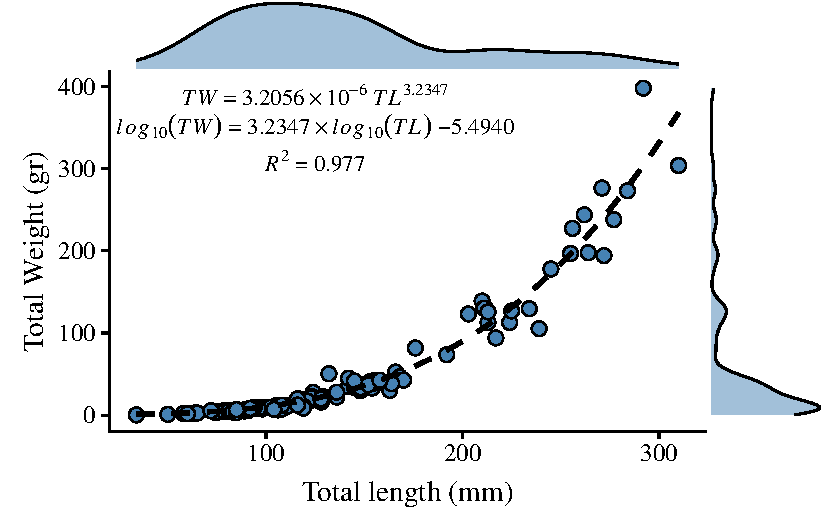
\includegraphics{Manuscript_files/figure-latex/unnamed-chunk-11-1.pdf}
%DIFDELCMD < %%%
\DIFdelendFL \DIFaddbeginFL 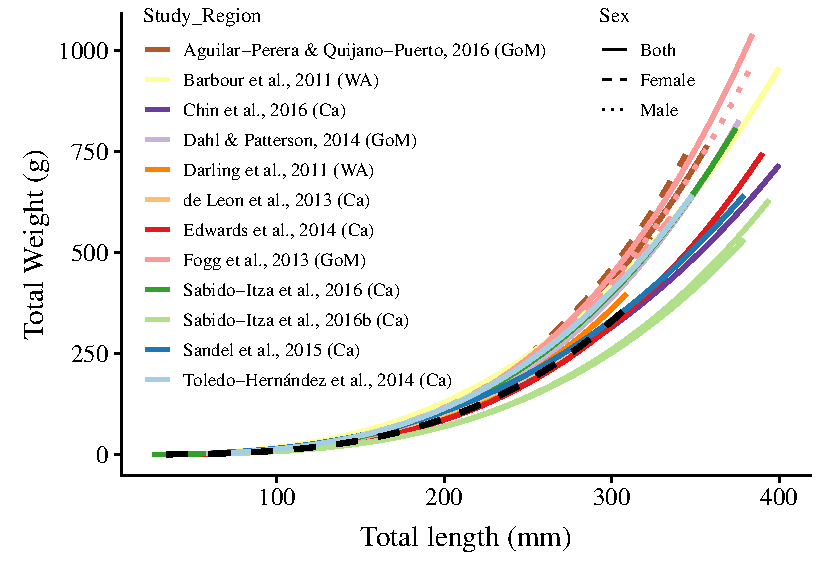
\includegraphics{Manuscript_files/figure-latex/fit2-1.pdf}
\DIFaddendFL \caption{\label{fig:all_allo}Length-weight relationships (n = 18) for 12
studies and this study. \DIFaddbeginFL \DIFaddFL{The curves are shown for the range of lengths
reported in each study (See Supplementary Table 2); when ranges were not
present, we use the ones found in this study (34 mm - 310 mm). }\DIFaddendFL Colors
indicate studies from which the parameters were extracted. Dotted,
dashed\DIFaddbeginFL \DIFaddFL{, }\DIFaddendFL and solid lines show models for males, females, and combined
sexes, respectively. The dashed black line represents the relationship
estimated in this study. \DIFaddbeginFL \DIFaddFL{There are two solid green lines for Sabido-Itza
et al, 2016b, one for each of the two sites for which they report
parameters. A log-log version of this figure is presented in Figure S4.}\DIFaddendFL }
\end{figure}

\begin{figure}
\centering
\DIFdelbeginFL %DIFDELCMD < 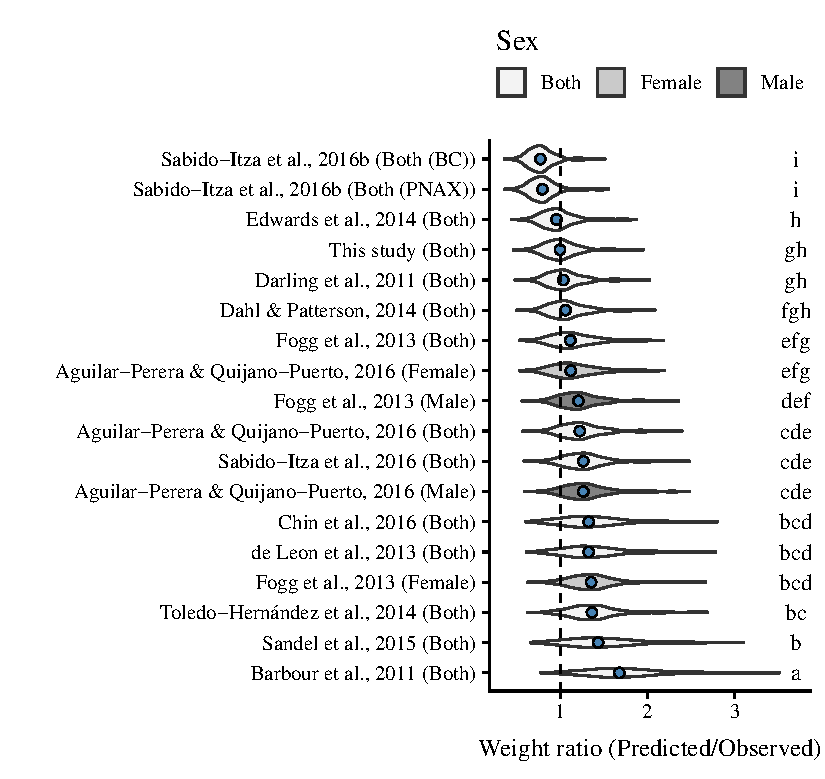
\includegraphics{Manuscript_files/figure-latex/unnamed-chunk-13-1.pdf}
%DIFDELCMD < %%%
\DIFdelendFL \DIFaddbeginFL 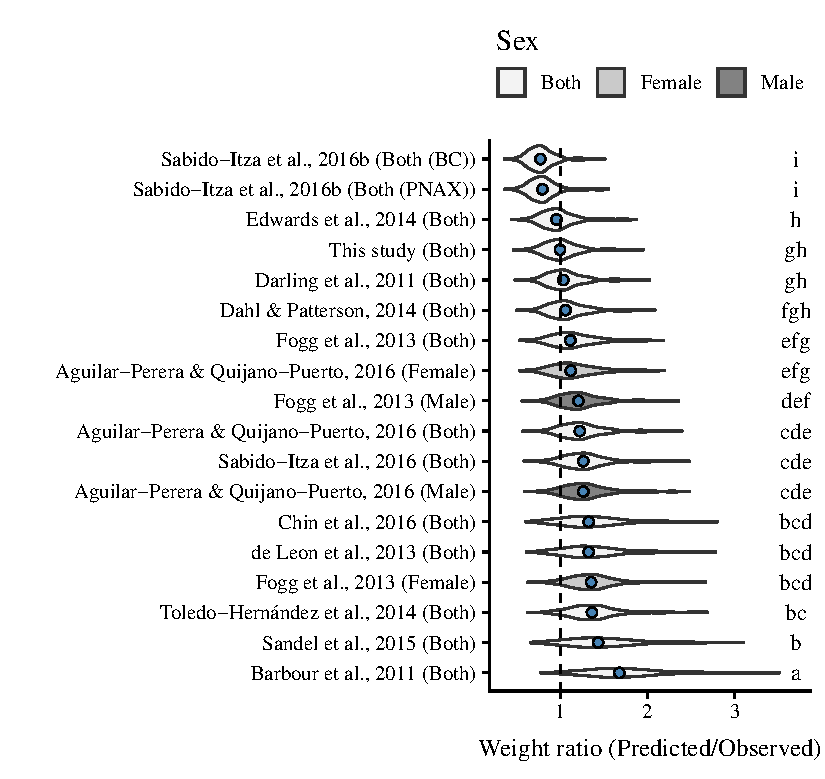
\includegraphics{Manuscript_files/figure-latex/pred_obs-1.pdf}
\DIFaddendFL \caption{\label{fig:bio_ratio}Violin plot of predicted-to-observed
weight ratios for 18 pairs of allometric parameters. Blue circles
indicate median values and \DIFdelbeginFL \DIFdelFL{Like }\DIFdelendFL \DIFaddbeginFL \DIFaddFL{like }\DIFaddendFL letters indicate values that do not
differ significantly. \DIFaddbeginFL \DIFaddFL{For Sabido-Itza et al, 2016b, BC and PNAX make
reference to Banco Chinchorro and Parque Nacional Arrecifes de Xcalak,
two sites for which they report parameters.}\DIFaddendFL }
\end{figure}

\clearpage

\section*{Discussion}

Our results suggest that lionfish exhibit highly variable allometric
relationships across the invaded range, and that this variation is
\DIFdelbegin \DIFdel{related to space}\DIFdelend \DIFaddbegin \DIFadd{spatially heterogeneous and relevant for management of the invasion}\DIFaddend .
Moreover, we \DIFdelbegin \DIFdel{shot }\DIFdelend \DIFaddbegin \DIFadd{show }\DIFaddend that the use of \emph{ex situ} parameters may lead to
highly biased weight estimates. Our comparison of observed weights to
those predicted with locally-informed parameters and \emph{ex situ}
parameters showed that weight can be overestimated by more than a
three-fold, and highlights the need to use local information. Here we
discuss the implications of our findings\DIFaddbegin \DIFadd{, possible shortcommings in our
analyses, }\DIFaddend and highlight potential future research directions.

\DIFaddbegin \DIFadd{Differences in length-weight relationships have traditionally been
highlighted as potential pitfalls to fishery management. For example,
\mbox{%DIFAUXCMD
\citet{wilson_2012} }\hspace{0pt}%DIFAUXCMD
show that small-scale variations in length-at-age
and fishing mortality in other Scorpaeniformes translate to differential
landings, effort, and catch per unit effort in the live fish fishery of
California, and that these differences must be taken into account in
management plans. The lionfish case poses the opposite scenario, where
the manager desires to eradicate the species. To accurately gauge both
the effectiveness of lionfish removal efforts and the resources needed
to successfully manage an invasion, we must acknowledge and understand
regional biological differences in important variables such as
allometric growth parameters.
}

\DIFaddend We detected substantial differences in weight-at-length between
organisms from the Caribbean, Gulf of Mexico, and \DIFdelbegin \DIFdel{North-Western
}\DIFdelend \DIFaddbegin \DIFadd{Western }\DIFaddend Atlantic.
Groupings of predicted-to-observed weight ratios \DIFaddbegin \DIFadd{identified in our
}\emph{\DIFadd{post hoc}} \DIFadd{testing }\DIFaddend aligned with the spatial distribution of the
examined studies, suggesting that these differences \DIFdelbegin \DIFdel{are }\DIFdelend \DIFaddbegin \DIFadd{may be }\DIFaddend mediated by
space. These regional allometric differences mirror similar patterns in
\DIFdelbegin \DIFdel{age-at-length }\DIFdelend \DIFaddbegin \DIFadd{length-at-age }\DIFaddend of lionfish across both their invaded and native regions
\citep{pusack_2016}. Variation may be driven by genetics or by
organisms' exposure to distinct environmental conditions. For example,
\citet{betancurr_2011} used mitochondrial DNA to demonstrate the
existence of two distinct population groups, identified as the
``Caribbean group'' and ``Northern Group'', and \citet{fogg_2015}
alternatively suggested that \DIFdelbegin \DIFdel{age-at-length }\DIFdelend \DIFaddbegin \DIFadd{length-at-age }\DIFaddend differences may be \DIFdelbegin \DIFdel{climate-driven.
}\DIFdelend \DIFaddbegin \DIFadd{driven by
the environment.
}

\DIFadd{We might be inclined to attribute all variation to the spatial origin of
these parameters. However, these were not only collected for different
locations, but also using a range of different sampling methods and at
different points in time (See Supplementary Table 2 for an extended
version of Table 1). While we are not able to evaluate how these factors
influence previous estimates (raw data from all studies would be
needed), it is certain that the lack of locally-calculated parameters
may induce significant bias when calculating weight from length
observations. }\DIFaddend Differences in weight-at-length could also reflect
differential energy input or usage, or a combination of both. \DIFdelbegin \DIFdel{Future research is needed to determine which processes are at work here.
}%DIFDELCMD < 

%DIFDELCMD < %%%
\DIFdel{Differences in }\DIFdelend \DIFaddbegin \DIFadd{The
magnitude of the bias and our lack of understanding of the source of
variation highlights the need to simultaneously collect }\DIFaddend length-weight
\DIFdelbegin \DIFdel{relationships have traditionally been
highlighted as potential pitfalls to fishery management.
For example,
\mbox{%DIFAUXCMD
\citet{wilson_2012} }\hspace{0pt}%DIFAUXCMD
show that small-scale variations in length-at-age
and fishing mortality in other Scorpaeniformes translate to differential
landings, effort, and catch per unit effort in the live fish fishery of California, and that these differences must be taken into account in
management plans. The lionfish case poses the opposite scenario, where
the manager desires to eradicate the
species. To accurately gauge both
the effectiveness of
lionfish removal efforts and the resources needed
to successfully manage an invasion, we must acknowledge and understand
regional biological differences in important variables such as
allometric growth parameters}\DIFdelend \DIFaddbegin \DIFadd{information across the invaded range to test for spatially-induced
patterns and link these to previously suggested environmental and
genetic structures. Such an endeavor would provide insights into
lionfish biology and better inform management.
}

\DIFadd{Applying parameters estimates to lengths outside the range of lengths
originally used to estimate the parameters may also induce error. Our
smallest observed organism was 34 mm in \(TL\), and only two studies
estimated parametrs with smaller organisms
\mbox{%DIFAUXCMD
\citep{sabidoitza_2016,edwards_2014}}\hspace{0pt}%DIFAUXCMD
. On the other hand, our largest
organism had a \(TL\) of 310 mm, which is well within the range of all
other studies (maximum observed lengths varied from 325 mm to 475 mm;
See Supplementary Table 2). Due to the power-function describing the
allometric relationship, the error is higher when extrapolation is done
for lengths that are larger than the maximum length used to estimate the
parameters. This means that not only must managers use locally-informed
data, but that these local data must also include the full range of
lengths present in the region to reduce error caused by extrapolation}\DIFaddend .

The results presented here have \DIFdelbegin \DIFdel{major }\DIFdelend \DIFaddbegin \DIFadd{fundamental }\DIFaddend implications for management.
For example, \citet{edwards_2014} simulated a lionfish culling program
under two scenarios, one using length-at-age and length-to-weight
parameters from North Carolina and one using parameters from Little
Cayman. Their results show that using different parameters caused up to
a four-year difference in the time required for the simulated lionfish
population to recover to 90\% of its initial biomass after removals
ceased. Here, we show that using one set of length-weight parameters
versus another for a given length can result in more than a threefold
under- or overestimation of total weight. These \DIFdelbegin \DIFdel{spatially-driven }\DIFdelend differences become
especially important when allocating resources for lionfish removal
programs, incentivizing lionfish fisheries as a source of alternative
livelihoods, or estimating ecosystem impacts. Research efforts focused
on invasive lionfish populations need to use parameters calculated for
their region to the extent possible, or at least use reasonable sets of
different parameters that provide upper and lower bounds in their
results.

\section*{\DIFdelbegin \DIFdel{Aknowledgements}\DIFdelend \DIFaddbegin \DIFadd{Acknowledgements}\DIFaddend }

The \DIFdelbegin \DIFdel{authors would like to thank }\DIFdelend thank Nils Van Der Haar and Michael Doodey from Dive Aventuras as
well as Guillermo Lotz-Cador who provided help to collect samples\DIFaddbegin \DIFadd{. We
are greateful for comments raised by the editor and two anonimous
reviewers, which significantly increased the quality of this work}\DIFaddend .

Conflict of Interest: The authors declare that they have no conflict of
interest.

\bibliography{references}

\end{document}